% !TeX root = ../libro.tex
% !TeX encoding = utf8
\chapter{Diseño, implementación y despliegue del simulador}
\section{Introducción}
Esta parte final está orientada a implementar los modelos y la resolución de sistemas de ecuaciones diferenciales mediante servicios, siguiendo Arquitectura Orientada a Servicios (\textit{Service Oriented Architectures, SOA}), con el objetivo de facilitar la integración de dichas funcionalidades en otras soluciones por parte de desarrolladores, además se ha implementado un simulador mediante tecnología web para mostrar la aplicación y utilidad de este trabajo de una forma mucho más gráfica y dinámica, con la posibilidad de cambiar los parámetros del edificio a nuestro gusto y ver cómo afectan estos a las distintas temperaturas del edificio.

Veremos el proceso y desarrollo del simulador, para el cual hemos utilizado tecnologías actuales que podremos encontrar en cualquier proyecto de desarrollo de las principales empresas hoy en día, además veremos los aspectos más importantes en el proceso de creación del backend y frontend, detallando todos los pasos que hemos seguido tanto en el diseño como implementación, mostraremos algunos ejemplos de casos de uso del simulador para comprobar su correcto funcionamiento comparándolo con la parte teórica, además, al final se discutirán posibles mejoras y actualizaciones que se podrían realizar sobre el proyecto a futuro.

El objetivo es que sea accesible para cualquier usuario, y para ello la interfaz será muy intuitiva y fácil de entender, además incluiremos en el \autoref{ap:apendice1} una pequeña guía de instalación y acceso del simulador, de tal forma que cualquiera pueda utilizarlo y probarlo.

Vamos a estudiar los diferentes tipos de arquitectura que, por lo general, siguen las aplicaciones, como cliente-servidor o monolítica, y veremos las características principales del modelo REST y RESTful, algunas ventajas y desventajas importantes y el papel que juegan dentro de las aplicaciones.
\section{Arquitectura de una aplicación}
La arquitectura de una aplicación describe cómo encajan sus piezas a alto nivel. Los desarrolladores utilizan muchos tipos de arquitecturas. Muchas de estas abordan características particulares del problema que se está resolviendo.

Por ejemplo, los sistemas basados en reglas se suelen utilizar para manejar situaciones complejas, en las que resolver un problema particular se pueda reducir a seguir un conjunto de reglas. Algunos sistemas de resolución de problemas utilizan este enfoque.
Algunas de las arquitecturas que veremos son:
\begin{itemize}
	\item Monolítica. Todas las funciones de la aplicación se implementan en un solo programa, lo que puede simplificar el desarrollo pero limita la flexibilidad y escalabilidad a medida que la aplicación crece.
	\item La arquitectura cliente-servidor separa las funciones de la aplicación en dos partes distintas: el cliente, que es la interfaz de usuario, y el servidor, que maneja el procesamiento y el almacenamiento de datos. Esta separación permite una mayor escalabilidad y distribución de tareas, pero puede introducir complejidad adicional en la comunicación entre el cliente y el servidor.
	\item La arquitectura orientada a servicios (SOA) es un enfoque en el que las diferentes funciones de la aplicación se exponen como servicios independientes, lo que permite una mayor reutilización y flexibilidad en el desarrollo de software empresarial.
	\item REST es un estilo arquitectónico para diseñar sistemas distribuidos que se basa en la idea de que cada recurso se identifica mediante un URI y se puede acceder y manipular a través de operaciones estándar de HTTP como GET, POST, PUT y DELETE. Esta arquitectura es especialmente adecuada para aplicaciones web y servicios web que requieren una alta escalabilidad y rendimiento.
\end{itemize}

En resumen, cada tipo de arquitectura tiene sus propias ventajas y desventajas, y la elección de la arquitectura depende por tanto de los requisitos y las restricciones específicas de cada proyecto.
\subsection{Arquitectura monolítica}
En una arquitectura monolítica, un solo programa hace todo. Muestra la interfaz de usuario, accede a los datos, procesa cualquier petición del servidor y hace todo lo que la aplicación necesite hacer.

Esta arquitectura tiene algunas desventajas significativas. En particular, las piezas del sistema están estrechamente vinculadas, por lo que no te ofrece mucha flexibilidad.

Una arquitectura monolítica también requiere comprender cómo encajan todas las piezas del sistema desde el principio del proyecto. Si cometes algún error en los detalles, el acoplamiento estrecho entre las piezas del sistema dificulta corregirlos más tarde.
Sin embargo, las arquitecturas monolíticas tienen algunas ventajas, debido a que todo está integrado en un solo programa, no es necesario tener una comunicación complicada a través de redes.
Las arquitecturas monolíticas también son útiles para aplicaciones pequeñas donde un solo programador o equipo está trabajando en el código.

Debido a estas ventajas que acabamos de comentar, es la arquitectura que hemos utilizado para realizar el simulador, ya que es más que suficiente para las necesidades del proyecto.
\subsection{Cliente-Servidor}
Una arquitectura cliente-servidor separa las piezas del sistema que necesitan usar una función particular (clientes) de las partes del sistema que proporcionan esas funciones (servidores). Eso desacopla las piezas de cliente y servidor del sistema para que los desarrolladores puedan trabajar en ellas por separado.
Por ejemplo, muchas aplicaciones dependen de una base de datos para mantener información, y la aplicación necesitará mostrar esa información en algún tipo de interfaz de usuario. Una forma de hacerlo sería integrar la base de datos directamente en la aplicación.
Un problema con este diseño es que múltiples usuarios no pueden usar los mismos datos. Puedes solucionar ese problema pasando a una arquitectura de dos niveles donde un cliente (la interfaz de usuario) está separado del servidor (la base de datos). Los clientes y el servidor se comunican a través de alguna red como una red de área local (LAN), red de área amplia (WAN) o Internet.
\begin{figure}[h!]
	\centering
	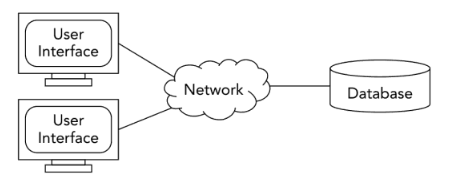
\includegraphics[width=0.8\textwidth]{2niveles}
	\caption{Arquitectura de $2$ niveles, donde el cliente está separado del servidor}
	\label{fig:2niveles}
\end{figure}
La arquitectura de dos niveles facilita el soporte de múltiples clientes con el mismo servidor, pero vincula estrechamente a clientes y servidores. Los clientes deben saber qué formato utiliza el servidor, y si cambias la forma en que el servidor presenta sus datos, necesitas cambiar el cliente para que coincida. Eso puede suponer un trabajo extra, especialmente al principio de un proyecto cuando las necesidades del cliente y del servidor no están completamente definidas. Podemos ver una imagen de la arquitectura de dos niveles en la \autoref{fig:2niveles}.

Otra opción es aumentar la separación entre los clientes y el servidor introduciendo otra capa entre los dos para crear una arquitectura de tres niveles.
En este caso, el nivel intermedio proporciona una separación entre los clientes y el servidor, la cual permite que diferentes equipos trabajen sin interferir demasiado entre sí.
Además de proporcionar separación, un nivel intermedio puede realizar otras acciones que hagan que los datos sean más fáciles de usar tanto para el cliente como para el servidor.

Se pueden definir otras arquitecturas multinivel que utilicen más de tres niveles si fuera necesario. Por ejemplo, un nivel de datos podría almacenar los datos, un segundo nivel podría calcular agregaciones y realizar otros cálculos sobre los datos, un tercer nivel podría usar técnicas de inteligencia artificial para hacer recomendaciones basadas en los datos del segundo nivel, y un cuarto nivel sería de presentación que permitiría a los usuarios ver los resultados.

Se puede encontrar más información acerca de la arquitectura monolítica y cliente-servidor en \cite{stephens2015beginning}.
\subsection{Arquitectura Orientada a Servicios, SOA}
En los últimos años, SOA ha recibido una atención creciente en línea con el movimiento hacia abordar los desafíos asociados con la mejora y mantenimiento de diversos entornos. Con el objetivo de modernizar el sistema de software de las organizaciones, la migración de un sistema heredado a un sistema basado en SOA se ha convertido en una tendencia predominante. \\
Son varios los beneficios de emplear SOA en el desarrollo de tecnologías líderes en el mundo actual, como \textit{Internet of Things} (IoT) y \textit{Cloud Computing} (CC), además de microservicios. Esto se debe a que SOA ofrece integración flexible y reutilización de servicios debido a su arquitectura modular basada en servicios. SOA también ofrece transparencia porque encapsula varias aplicaciones y fuentes de datos en forma de caja negra. De esta manera, un conjunto integrado de recursos de Tecnologías de la Información (TI) aún podría ser accesible a pesar de la existencia de diversas tecnologías, códigos de lenguaje, funcionalidades y plataformas.

Aunque no hay una definición clara de SOA, en \cite{soa} se define como un concepto arquitectónico que promueve el acoplamiento flexible, la reutilización, la interoperabilidad, la agilidad, la eficiencia, con un enfoque en descomponer cada proceso empresarial en bloques más pequeños de tareas y funciones como servicios. Estos servicios están bien definidos y organizados y sirven como unidades independientes de funcionalidad empresarial estándar que están conectadas entre sí para crear un proceso empresarial unificado.

En \cite{soa} se indican varios estudios que afirman que la combinación de SOA con otras tecnologías podría proporcionar más beneficios para las organizaciones. Podría integrarse con nuevas tecnologías médicas, agentes inteligentes, tecnologías inalámbricas, identificación por radiofrecuencia (RFID) y procedimientos operativos de Internet para establecer nuevas automatizaciones para el proceso empresarial. Además, los requisitos de IoT podrían cumplirse mediante el enfoque SOA, ya que puede proporcionar medición de rendimiento, detección de ataques de seguridad e inteligencia empresarial.

\subsection{REST y RESTful}
REST (Representational State Transfer) es un conjunto de criterios de diseño para desarrollar proyectos basados en recursos, que cambió por completo la ingeniería del software y es un concepto fundamental para el desarrollo de cualquier sistema (aplicaciones móviles, sistemas industriales, empresas, negocios, etc...).
\begin{figure}[h!]
	\centering
	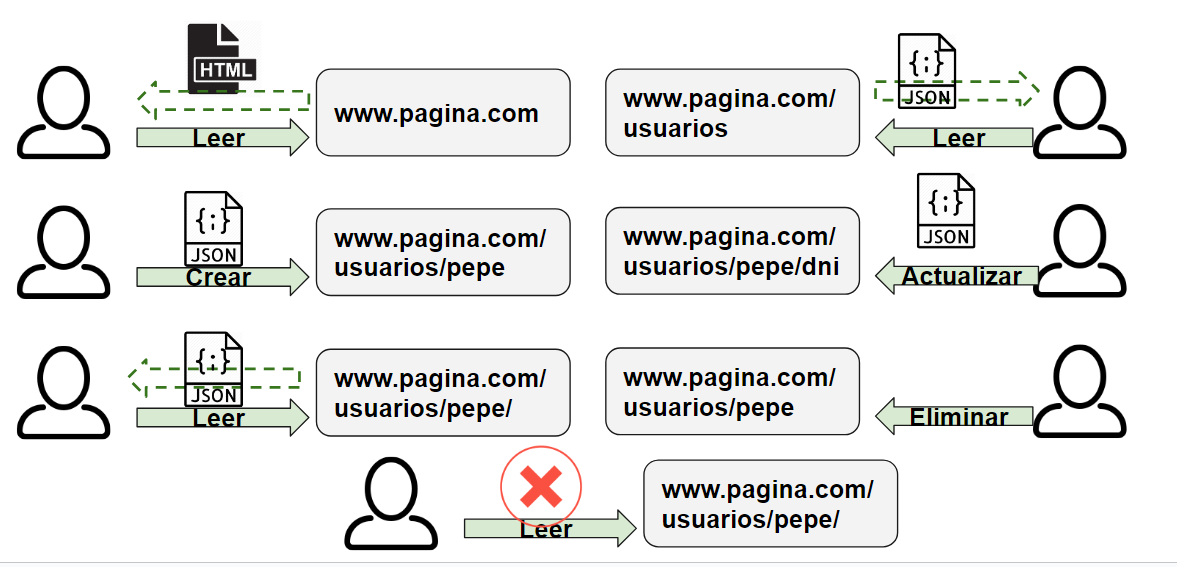
\includegraphics[width=0.9\textwidth]{rest}
	\caption{Ejemplo de las operaciones de transferencia de estado}
	\label{fig:operaciones}
\end{figure} RESTful se suele utilizar para referirse a los servicios web de ejecución de una arquitectura REST.
El objetivo de REST es definir recursos, modificarlos e intercambiar la representación de estos en un formato concreto: XML, JSON, HTML, texto plano, etc... Estos recursos se identifican de forma única mediante un URI \textit{(Uniform Resource Identifier)} y son accesibles globalmente, además se construyen de forma dinámica. Estos recursos se pueden manipular a través de operaciones estándar de HTTP como pueden ser GET, POST, PUT o DELETE que sirven para leer, actualizar, crear y eliminar, respectivamente.
En la \autoref{fig:operaciones} podemos ver un ejemplo de uso de las distintas operaciones.

Los recursos se pueden clasificar en dos tipos principalmente:
\begin{itemize}
	\item Entrypoint: URL de un sitio web para visualizar el contenido, están diseñados para interactuar con el usuario final.
	\item Endpoint: URL de una API que responde a una petición, a diferencia del entrypoint, no están diseñados para interactuar con el usuario final.
\end{itemize}
Las principales ventajas que nos ofrece el uso de REST son:
\begin{itemize}
	\item Separación entre cliente y servidor que nos permite distinguir entre la interfaz de usuario del servidor y del almacenamiento de datos, además de mejorar la portabilidad con otros proyectos.
	\item Visibilidad, fiabilidad y escalabilidad gracias a la separación entre cliente y servidor añadiendo nuevos recursos.
	\item El desarrollo orientado a recursos es muy modular, al usar encapsulación y reusabilidad.
	\item La interfaz de acceso a los diferentes recursos es universal, debido al uso de HTTP, JSON/XML y ser independiente de cualquier plataforma.
	\item Es uno de los conceptos más ampliamente usados actualmente para el desarrollo, prácticamente cualquier sistema actual usa tecnología REST/RESTful en su backend.
\end{itemize}
Sin embargo, también existen algunas desventajas:
\begin{itemize}
	\item Es necesario abordar problemas de una forma distinta, cambiando el modo de pensar.
	\item Al principio requiere un mayor tiempo de desarrollo y más conocimientos que otros modelos clásicos de servicios web.
\end{itemize}
\section{Tecnologías utilizadas}
A continuación vamos a enumerar y explicar los principales motivos y características acerca de las tecnologías que hemos utilizado, incluyendo el enlace a sus páginas web oficiales. Empezamos por las que hemos requerido para desarrollar el backend:
\begin{itemize}
	\item \href{https://www.python.org}{Python}. Además de porque tiene una comunidad muy amplia, la cual nos permite encontrar feedback rápidamente sobre cualquier duda o problema que tengamos, es uno de los lenguajes más utilizados para ciencia de datos, IA y cálculo, por lo que existen muchas librerías para simplificar la implementación de nuestros sistemas de ecuaciones diferenciales. Aunque otra opción es utilizar Java o en $C$++, sería más complejo realizar el cálculo de las ecuaciones diferenciales además del manejo de los datos, así que por las necesidades del proyecto hemos decidido utilizar Python. Las principales bibliotecas que hemos utilizado para el cálculo matemático son \href{https://numpy.org}{Numpy} y \href{https://scipy.org}{Scipy}.
	\item \href{https://flask.palletsprojects.com/en/3.0.x/}{Flask}. Es un framework para Python muy popular utilizado comúnmente para crear aplicaciones web, y sobre todo, servicios web. Nos hemos decantado por su uso debido al hecho de ser gratuito y de código abierto, además de su sencillo uso.
	\item \href{https://www.json.org/json-es.html}{JSON}. Notación estándar para el intercambio de información entre los servicios y las aplicaciones. Está basado en un subconjunto del lenguaje JavaScript, y una característica muy importante es que no depende del lenguaje que se utilice, por lo que es ideal para el intercambio de datos.
	\item \href{https://www.openapis.org}{OpenAPI}. Es una notación estándar para describir y compartir con otros usuarios (desarrolladores, comunidad) nuestro servicio web (resolución de sistemas de ecuaciones diferenciales).
\end{itemize}
En cuanto al desarrollo del frontend hemos utilizado:
\begin{itemize}
	\item \href{https://es.react.dev}{React}. Es una de las librerías más populares de JavaScript, está diseñada para crear interfaces de usuario con el objetivo de facilitar el desarrollo de aplicaciones en una sola página. Tiene un alto rendimiento y permite infundir código HTML con JavaScript. Aplicaciones muy populares como Facebook, Netflix, DropBox, Instagram o Paypal usan React, y es por ello que es tan importante y he querido familiarizarme con ella en este trabajo. Además, es mantenida por Facebook y la comunidad de software libre.
	\item \href{https://www.highcharts.com}{Highcharts}. Es una librería escrita en JavaScript para generar gráficos interactivos en aplicaciones web, soporta una gran variedad de gráficos y en nuestro caso la utilizaremos para mostrar el resultado final.
	\item \href{https://getbootstrap.com}{Bootstrap}. Es un framework que permite a los desarrolladores web darle forma a un sitio web y adaptarlo a las necesidades de los usuarios, nosotros lo hemos utilizado para mejorar el diseño de la página.
	\item \href{https://ant.design}{Ant Design}. Es una biblioteca React UI (User Interface), que como su nombre indica, permite construir interfaces de usuario con un elegante diseño, la hemos compaginado con Bootstrap para mejorar el diseño de la página.
\end{itemize}
En el diagrama de la \autoref{fig:arquitectura} podemos ver la arquitectura que sigue el simulador junto con los logos de las principales tecnologías que hemos utilizado tanto para el frontend como para el backend.
\begin{figure}[h!]
	\centering
	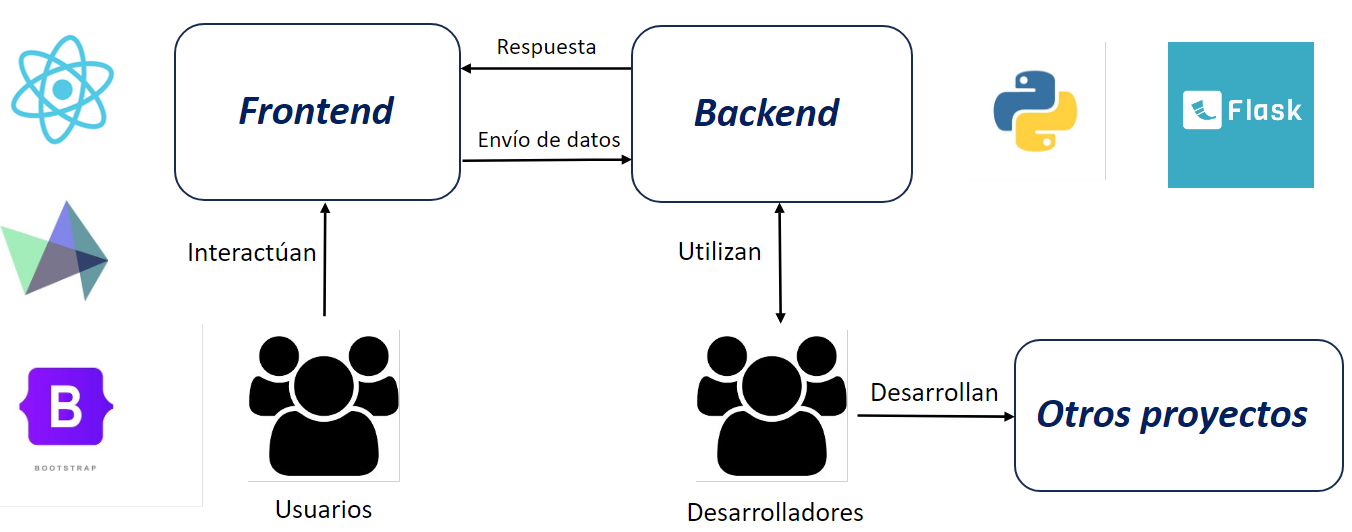
\includegraphics[width=\textwidth]{diagrama}
	\caption{Arquitectura del simulador}
	\label{fig:arquitectura}
\end{figure}
\section{Frontend}
\subsection{Idea inicial del diseño}
En la \autoref{fig:mockup} podemos ver un wireframe del diseño propuesto para el frontend antes de realizar la implementación. Para recoger los datos y parámetros del edificio hemos decidido utilizar un cuestionario sencillo, y justo debajo tendrá un botón para enviar los datos a la API.

En el lado derecho tendremos un logo o nombre del simulador con el objetivo de darle una seña de identidad al proyecto, y justo debajo una gráfica con la solución al problema, es decir, las temperaturas de las habitaciones internas del edificio, que se mostrarán como respuesta de la API cuando le demos al botón de enviar. Por último un botón para descargar los resultados en formato JSON, por si algún desarrollador quiere utilizarlo en otro proyecto.
\begin{figure}[h!]
	\centering
	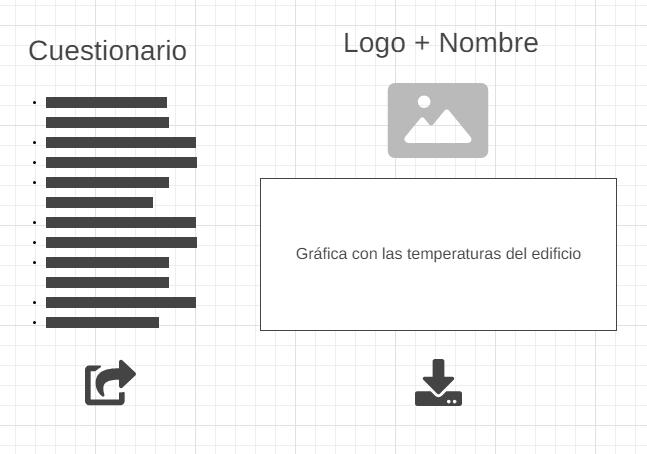
\includegraphics[width=0.9\textwidth]{mockup}
	\caption{Idea principal del diseño del simulador}
	\label{fig:mockup}
\end{figure}
\subsection{Desarrollo y diseño}
El objetivo principal del frontend es tener una herramienta web, visual y atractiva, que mediante una serie de parámetros, nos permita obtener los valores correspondientes a la resolución de nuestros sistemas de ecuaciones diferenciales, para que cualquier tipo de usuario pueda hacer uso de esta herramienta sin tener un conocimiento experto relacionado con las matemáticas ni la informática.
\begin{figure}[h!]
	\centering
	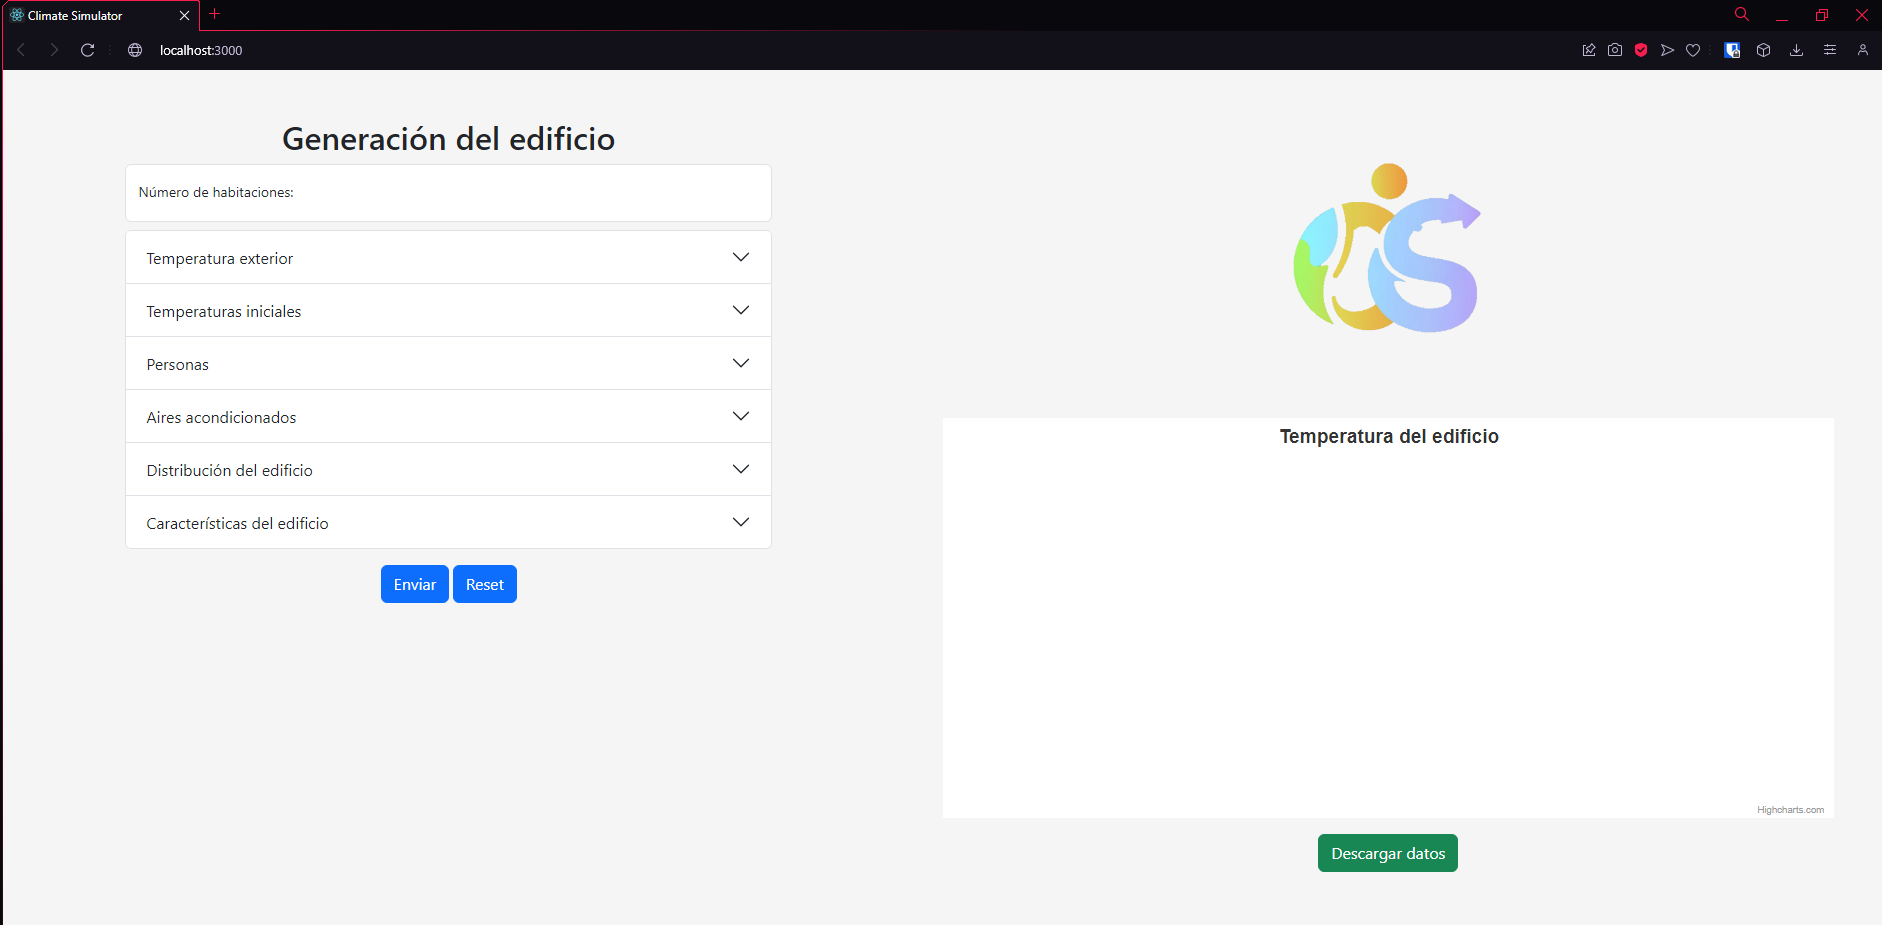
\includegraphics[width=\textwidth]{pag_web}
	\caption{Frontend del simulador}
	\label{fig:pag_web}
\end{figure}

Nada más abrir la página nos encontramos con el aspecto que podemos ver en la \autoref{fig:pag_web}, donde a la izquierda tenemos un formulario dinámico que nos permite generar el edificio con todos los parámetros necesarios, y es que los campos del formulario varían en tiempo real según el número de habitaciones, esto es posible gracias a que estamos utilizando React. Para mejorar el diseño del formulario hemos utilizado tanto Ant Design como Bootstrap.
\begin{figure}[h!]
	\centering
	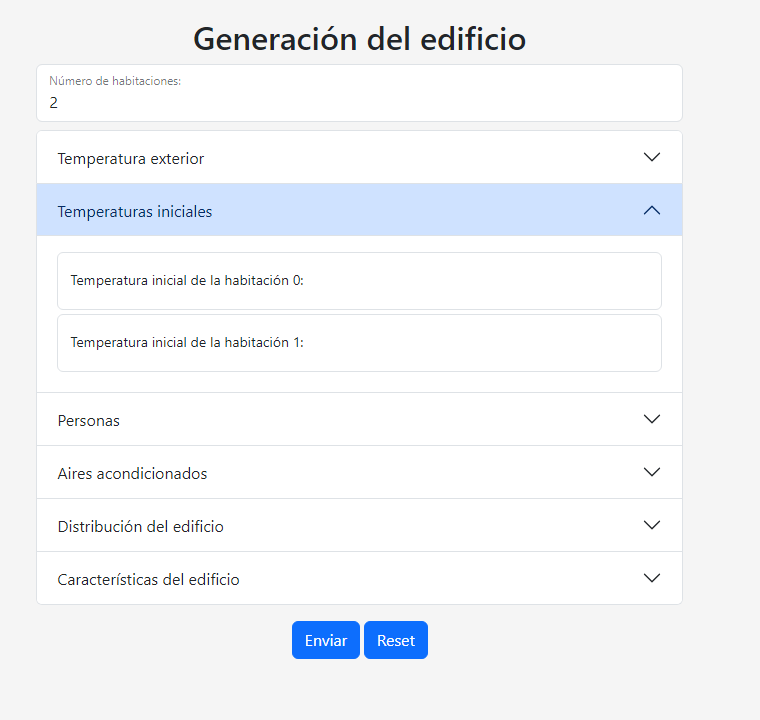
\includegraphics[width=0.7\textwidth]{formulario_2habs}
	\caption{Formulario introducir $2$ habitaciones}
	\label{fig:form_2habs}
\end{figure}
En la \autoref{fig:form_2habs} podemos ver cómo se incluyen $2$ habitaciones en el desplegable al haber introducido que el edificio tendrá $2$ habitaciones, y si cambiamos el número de habitaciones, el formulario cambia dinámicamente.

Para añadir la temperatura exterior, hemos incluido dos opciones, que podremos cambiar haciendo click en la barra superior del campo:
\begin{figure}[h!]
	\centering
	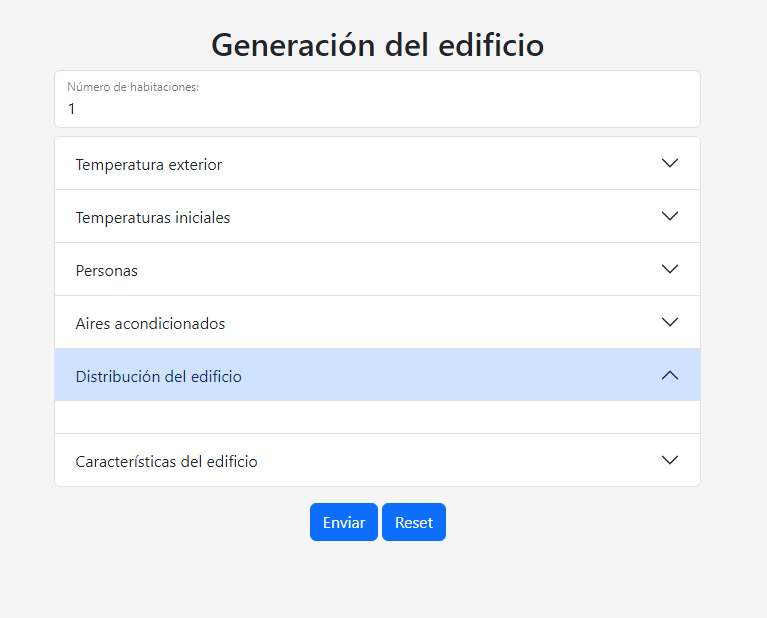
\includegraphics[width=0.75\textwidth]{una_hab}
	\caption{Formulario con $1$ habitación}
	\label{fig:una_hab}
\end{figure}
\begin{itemize}
	\item Opción $1$: Aquí podremos incluir directamente la función que tendrá la temperatura exterior durante las $24$ horas, está pensada para usuarios expertos en el tema. La función debe ser leída por la biblioteca $NumPy$ de Python, luego tendremos que usar expresiones como por ejemplo: $5 - 10*np.cos(t*np.pi/12)$
	\item Opción $2$: Podremos indicar la temperatura media del día y además cuánta variación tendrá, por ejemplo, si ponemos temperatura media de $10 \celsius$, y variación de $5$, entonces la temperatura variará entre $5 \celsius -15 \celsius$ grados, esta opción está pensada para que cualquier tipo de usuario pueda introducir la temperatura externa, sin necesidad de tener un conocimiento experto.
\end{itemize}

Otro detalle a tener en cuenta es que si ponemos sólo una habitación, no nos aparecerá la distribución del edificio, ya que no tendría sentido, como podemos ver en la \autoref{fig:una_hab}.

Al final tenemos dos botones tanto para enviar el formulario y obtener inmediatamente la gráfica con las temperaturas a la derecha, o para resetear el formulario por si queremos empezar de nuevo a crear el edificio.
\begin{figure}[h!]
	\centering
	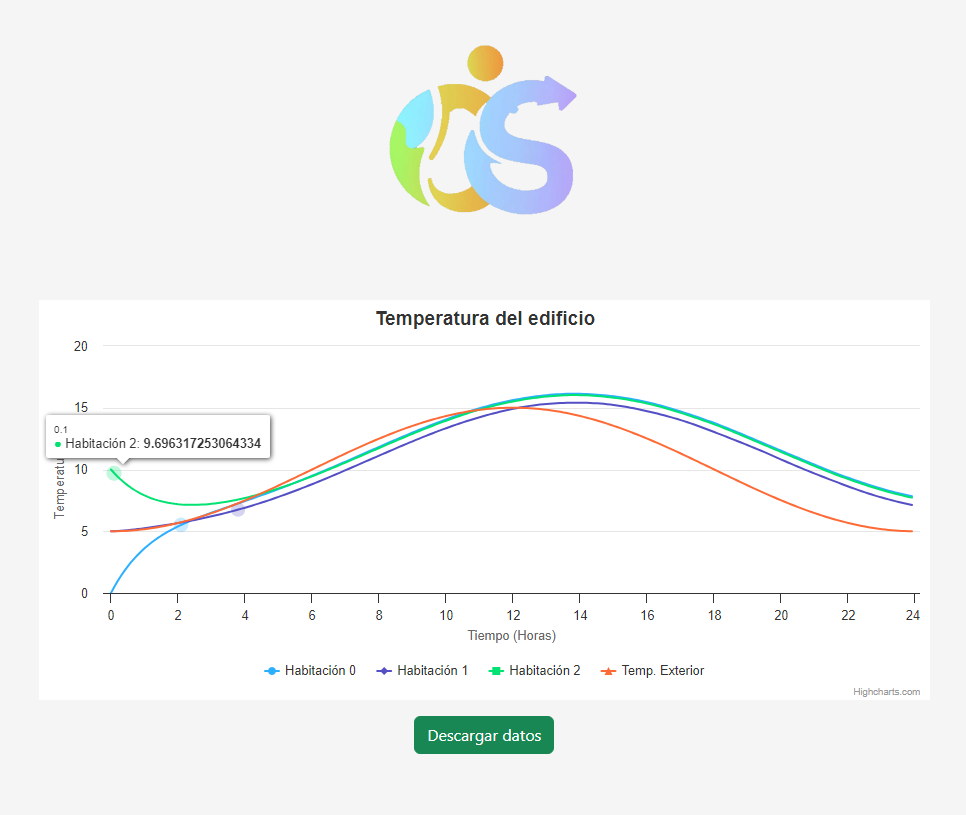
\includegraphics[width=\textwidth]{parte_derecha}
	\caption{Parte derecha de la página}
	\label{fig:parte_derecha}
\end{figure}

Ahora pasando a la parte derecha, tenemos en primer lugar el logo que hemos decidido añadir a la página, esto le aporta una identidad al proyecto aparte de ser más atractivo, justo debajo tenemos la solución al problema, es decir, una gráfica que hemos incluido gracias a Highcharts donde podemos ver las temperaturas de cada habitación, además de la temperatura externa para cada momento del día, y si pasamos el cursor por encima podemos ver el valor numérico de la temperatura en una hora determinada, todo esto se muestra en la \autoref{fig:parte_derecha}.

Por último, hemos incluido justo debajo un botón verde que nos permite descargar los datos de las temperaturas obtenidas en formato JSON, esta es una funcionalidad muy interesante que nos permite utilizar los resultados como posible entrada para otro programa por si fuesen necesarios.

\section{Desarrollo del Backend}
Vamos a utilizar un estilo RESTful, ya que es el más utilizado hoy en día, esto quiere decir que nuestro servicio web implementa una arquitectura de REST, que sirve para estandarizar comunicaciones web entre sistemas, logrando que se entiendan mucho mejor entre ellos. Se basa en que el cliente envía peticiones para recuperar o modificar recursos, y el servidor responde con el resultado, que puede ser con los datos que hemos pedido o el estado de la petición.

Todo el desarrollo lo hemos realizado utilizando el lenguaje de programación Python, y nos hemos servido de Flask para crear el servicio web.

El objetivo principal de nuestra API es resolver sistemas de ecuaciones diferenciales, para ello recibimos del servidor web las ecuaciones, las condiciones iniciales y la función que representa la temperatura exterior del edificio, y devuelve un vector formado por:
\begin{itemize}
	\item Un vector con los puntos que representarán el tiempo en el eje $X$ (de $0$ a $24$ horas).
	\item Un vector en el que cada componente contiene otro vector con las temperaturas de cada habitación en cada instante de tiempo (los puntos del primer vector).
	\item Un último vector formado por la temperatura externa en cada instante de tiempo.
\end{itemize} 
Esto se lo mandamos como respuesta al frontend, donde se construirá la gráfica final con los resultados obtenidos.

\begin{figure}[h!]
	\centering
	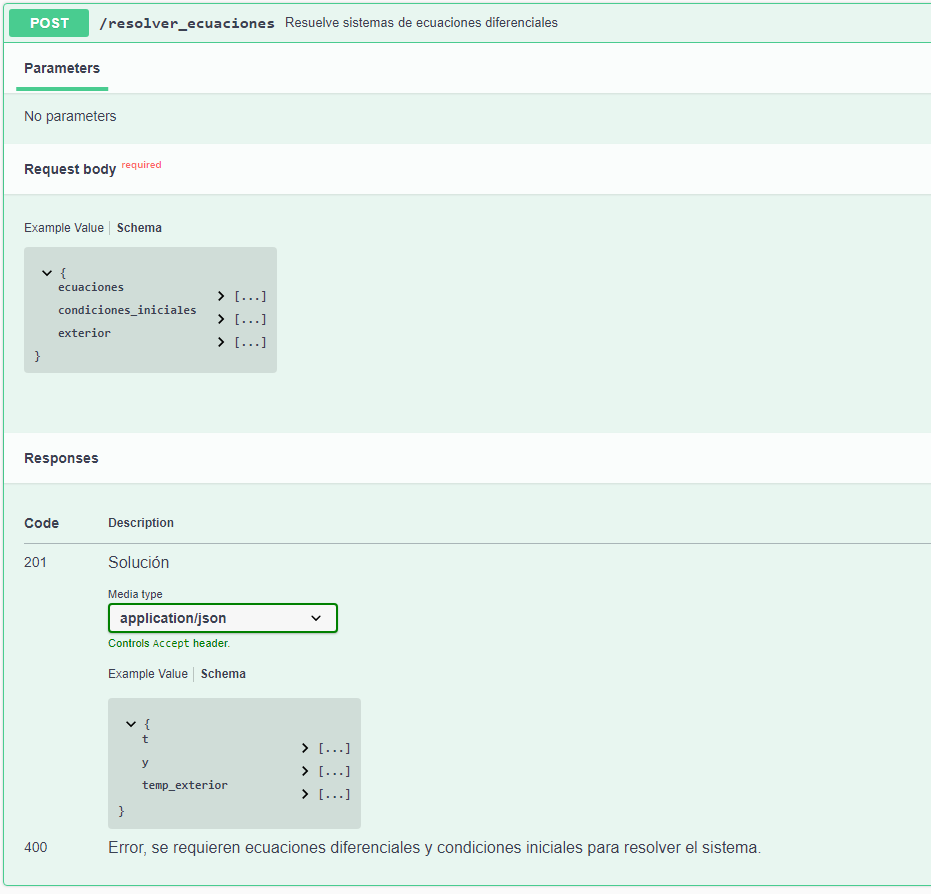
\includegraphics[width=\textwidth]{openapi}
	\caption{Especificación OpenAPI}
	\label{fig:openapi}
\end{figure}

Además, vamos a añadir el estándar de OpenAPI, que nos permite visualizar los métodos de la API para que cualquier programador o persona interesada pueda ver de forma esquemática el uso y funcionamiento detallado de cada uno de los métodos. Un detalle muy importante es que es independiente del lenguaje de programación con el que esté desarrollada la API. En la \autoref{fig:openapi} podemos ver cómo queda la documentación, la cual es accesible para todo el mundo. Podemos ver el archivo con la especificación OpenAPI completa en \autoref{ap:especificacion}.

\section{Casos de uso}
\subsection{Ejemplo con 3 habitaciones que vimos en la \autoref{fig:edif3}}
Siguiendo el modelo de edificio que tomamos en el ejemplo de la \autoref{fig:edif3}, vamos a rellenar el formulario con los siguientes datos:
\begin{itemize}
	\item Número de habitaciones: $3$
	\item Temperatura exterior: $5 - 10\cdot cos(t\cdot \pi/12)$
	\item Temperatura inicial de las habitaciones: $20,10,15$
	\item Cantidad de personas en las habitaciones: $1,10,0$
	\item Aires acondicionados en las habitaciones $0$ y $2$
	\item Distribución del edificio: 
	\begin{itemize}
		\item Habitaciones contiguas a la habitación $0$: $1,2$
		\item Habitaciones contiguas a la habitación $1$: $0$
		\item Habitaciones contiguas a la habitación $2$: $0$
	\end{itemize}
	\item Características del edificio:
	\begin{itemize}
		\item Constante de transferencia entre habitaciones: $5$
		\item Constante de transferencia con el exterior: $3$
		\item Calor generado por el aire acondicionado: $-8\celsius / 5h$
	\end{itemize}
\end{itemize}
Al introducir los datos en el formulario y hacer click en el botón Enviar, obtenemos la solución al problema, la cual coincide con la que vimos en \autoref{fig:graf_sol3}:
\begin{figure}[h!]
	\centering
	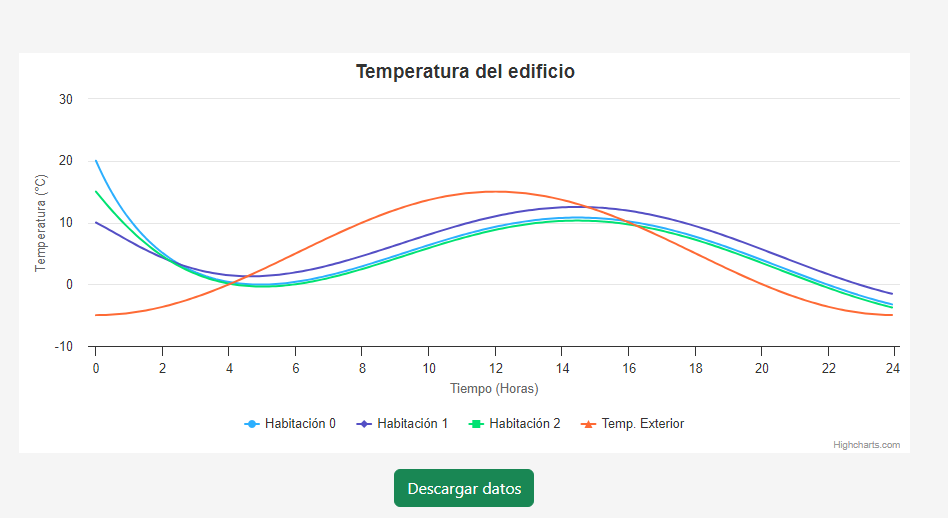
\includegraphics[width=\textwidth]{uso1}
	\caption{Temperaturas internas del edificio}
	\label{fig:caso1}
\end{figure}
\subsection{Ejemplo con 6 habitaciones}
Vamos a diseñar un nuevo edificio algo más elaborado, que constará de 6 habitaciones y seguirá la estructura que podemos ver en la \autoref{fig:edificio6}.
\begin{figure}[h!]
	\centering
	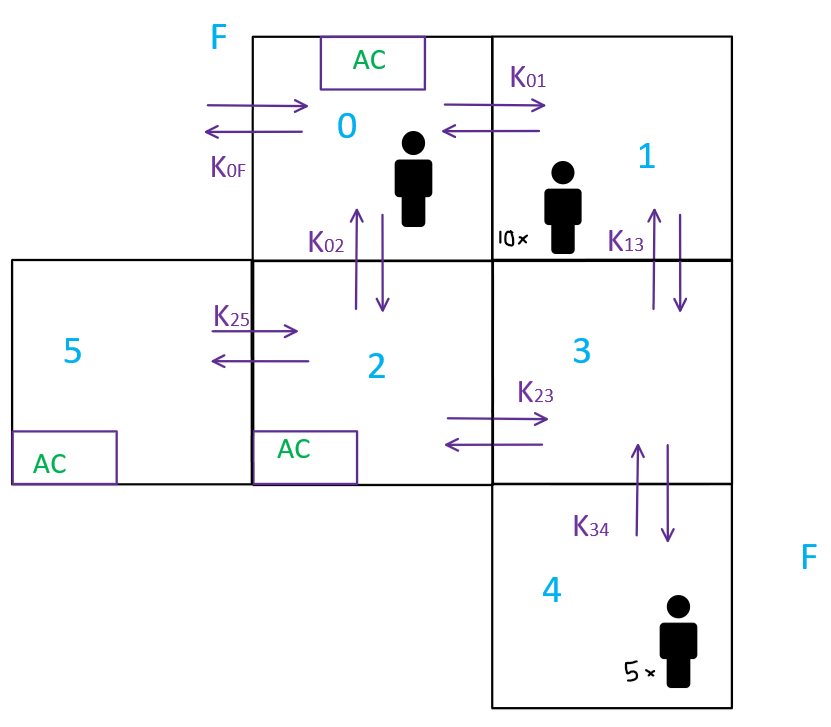
\includegraphics[width=0.8\textwidth]{edificio_6habs}
	\caption{Estructura del edificio con 6 habitaciones}
	\label{fig:edificio6}
\end{figure}
Vamos a introducir los siguientes datos en el formulario que corresponden con nuestro edificio:
\begin{itemize}
	\item Número de habitaciones: $6$
	\item Temperatura exterior: $20 - 15\cdot cos(t\cdot \pi/12)$
	\item Temperatura inicial de las habitaciones: $20,10,15,5,5,12$
	\item Cantidad de personas en las habitaciones: $1,10,0,0,5,0$
	\item Aires acondicionados en las habitaciones $0$, $2$ y $5$
	\item Distribución del edificio: 
	\begin{itemize}
		\item Habitaciones contiguas a la habitación $0$: $1,2$
		\item Habitaciones contiguas a la habitación $1$: $0,3$
		\item Habitaciones contiguas a la habitación $2$: $0,3,5$
		\item Habitaciones contiguas a la habitación $3$: $1,2,4$
		\item Habitaciones contiguas a la habitación $4$: $3$
		\item Habitaciones contiguas a la habitación $5$: $2$
	\end{itemize}
	\item Características del edificio:
	\begin{itemize}
		\item Constante de transferencia entre habitaciones: $3$
		\item Constante de transferencia con el exterior: $8$
		\item Calor generado por el aire acondicionado: $-4\celsius / h$
	\end{itemize}
\end{itemize}
Al introducir los datos en el formulario y hacer click en el botón Enviar, obtenemos la solución al problema, como podemos ver en la \autoref{fig:caso2}. Podemos observar que el edificio tiene un gran aislamiento con el exterior, y es por ello que las temperaturas de las habitaciones no se ven prácticamente influenciadas por la temperatura exterior, además de las altas temperaturas exteriores y tener un aire acondicionado que genera bastante frío, podríamos estar ante un escenario típico de verano.
\begin{figure}[h!]
	\centering
	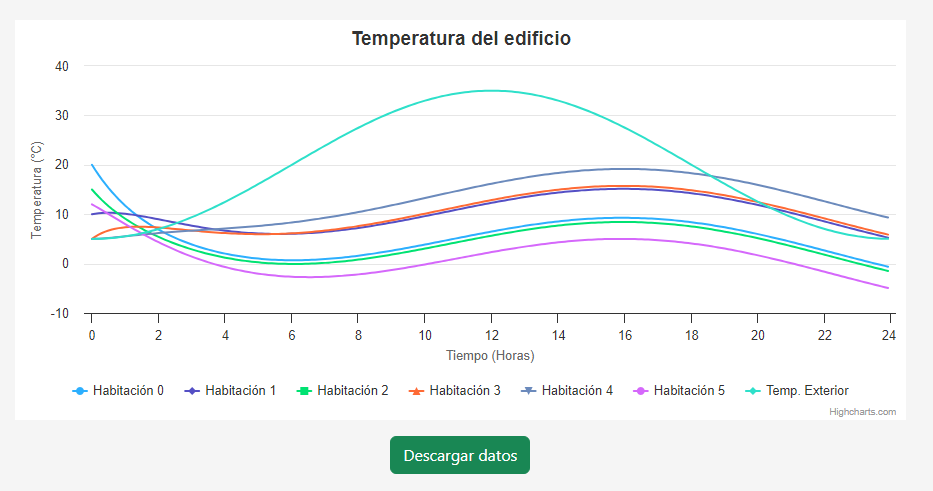
\includegraphics[width=\textwidth]{sol_6habs}
	\caption{Temperaturas internas del edificio con 6 habitaciones}
	\label{fig:caso2}
\end{figure}




\endinput
%------------------------------------------------------------------------------------
% FIN DEL CAPÍTULO. 
%----------------------------------------------------------------------------------
-